%Version 3.1 December 2024
% See section 11 of the User Manual for version history
%
%%%%%%%%%%%%%%%%%%%%%%%%%%%%%%%%%%%%%%%%%%%%%%%%%%%%%%%%%%%%%%%%%%%%%%
%%                                                                 %%
%% Please do not use \input{...} to include other tex files.       %%
%% Submit your LaTeX manuscript as one .tex document.              %%
%%                                                                 %%
%% All additional figures and files should be attached             %%
%% separately and not embedded in the \TeX\ document itself.       %%
%%                                                                 %%
%%%%%%%%%%%%%%%%%%%%%%%%%%%%%%%%%%%%%%%%%%%%%%%%%%%%%%%%%%%%%%%%%%%%%

\documentclass[pdflatex,sn-mathphys-num]{sn-jnl}

%%%% Standard Packages
\usepackage{graphicx}%
\usepackage{multirow}%
\usepackage{amsmath,amssymb,amsfonts}%
\usepackage{amsthm}%
\usepackage{mathrsfs}%
\usepackage[title]{appendix}%
\usepackage{xcolor}%
\usepackage{textcomp}%
\usepackage{manyfoot}%
\usepackage{booktabs}%
\usepackage{algorithm}%
\usepackage{algorithmicx}%
\usepackage{algpseudocode}%
\usepackage{listings}%
\usepackage{siunitx}%
\usepackage{bm}%
\usepackage{placeins}%
\usepackage{hyperref}%
\usepackage{caption}
\usepackage{subcaption}
\usepackage{float}

%%%% Theorem styles as per the template
\theoremstyle{thmstyleone}%
\newtheorem{theorem}{Theorem}%
\newtheorem{proposition}[theorem]{Proposition}%

\theoremstyle{thmstyletwo}%
\newtheorem{example}{Example}%
\newtheorem{remark}{Remark}%

\theoremstyle{thmstylethree}%
\newtheorem{definition}{Definition}%

\raggedbottom

\begin{document}

\title[A Dual-Branch Network with Hierarchical Feature Alignment]{A Dual-Branch Network with Hierarchical Feature Alignment for Fine-Grained Image Classification via Information Complementarity and Redundancy Suppression}

\author*[1]{\fnm{XX} \sur{XX}}
\affil*[1]{\orgdiv{Department of CSE(AIML)}, \orgname{Institute of Engineering and Management}, \orgaddress{\city{Kolkata}, \postcode{700091}, \country{India}}}

\abstract{
Fine-grained image classification aims to distinguish visually similar subcategories within the same basic category, and remains challenging due to small inter-class differences and large intra-class variations. Although recent deep models have achieved promising results, their performance often degrades under limited training data because discriminative representations are difficult to learn reliably. Existing approaches have attempted to incorporate hierarchical semantic cues, such as coarse-grained labels, to facilitate fine-grained recognition. However, most of them rely on simple cascaded, parallel, or feature-fusion designs, without explicitly modeling cross-level semantic dependency or suppressing feature redundancy across branches. To address these issues, this paper proposes a hierarchical feature enhancement network (HFENet) for data-limited fine-grained image classification. The core idea is to achieve hierarchical feature alignment through cross-branch interaction between coarse-grained and fine-grained representations. Specifically, a cross-branch attention mechanism is introduced to dynamically transfer semantic guidance from the coarse branch to the fine branch, while an orthogonality regularization term is employed to reduce redundant representations and encourage complementary feature learning. In addition, a hierarchical Kullback--Leibler divergence is incorporated into the optimization objective to improve semantic consistency between branches. Experiments on CIFAR-100 show that the proposed method achieves accuracies of 70.8\%, 77.2\%, 80.5\%, and 82.7\% under 30\%, 50\%, 80\%, and 100\% training ratios, respectively. The results indicate that HFENet provides consistent improvements over the baseline dual-branch model and several representative comparison methods, especially in low-data settings. Ablation studies and visualization results further confirm the effectiveness of the proposed hierarchical alignment and redundancy suppression mechanisms.
}

\keywords{Fine-grained image classification, Hierarchical feature alignment, Cross-branch attention, Orthogonality regularization, Complementary representation learning, Data-efficient learning}

\maketitle

\section{Introduction}
\label{sec:introduction}

Fine-grained image classification (FGIC) aims to distinguish visually similar subcategories within the same basic-level category. 
Compared with generic image classification, FGIC is more challenging due to subtle inter-class differences and large intra-class variations. 
These challenges become more severe under limited training data, where models are prone to overfitting and often fail to learn robust discriminative representations.

Existing studies have attempted to improve FGIC performance by introducing attention mechanisms, multi-branch architectures, and hierarchical semantic supervision. 
Although these methods have shown promising results, two limitations still remain. 
First, the semantic relationship between coarse-grained and fine-grained representations is often not explicitly modeled. 
Most existing hierarchical methods simply concatenate or sum features from different levels without modeling the conditional dependency that coarse semantics should guide fine-grained discrimination. 
Second, multi-branch designs may introduce redundant representations, which weakens the effectiveness of hierarchical learning. 
When two branches are trained jointly without constraints, they tend to capture overlapping information rather than complementary cues, leading to suboptimal feature utilization.

To address these issues, we propose a Hierarchical Feature Enhancement Network (HFENet) for fine-grained image classification. 
The proposed method is organized around a single central idea, namely hierarchical feature alignment for coarse-to-fine representation learning. 
Based on this idea, we introduce two key mechanisms and one auxiliary optimization strategy. 
First, a cross-branch attention (CBA) module is designed to transmit coarse-level semantic guidance to the fine-grained branch through conditional feature modulation. 
Second, an orthogonality regularization term is introduced to suppress cross-branch redundancy and encourage complementary representation learning. 
In addition, a hierarchical KL consistency objective is employed as an auxiliary optimization term to improve training-level semantic coherence between coarse- and fine-grained predictions. 
Together, these components enable the network to learn more structured, discriminative, and data-efficient representations.

The main contributions of this work are summarized as follows:
\begin{itemize}
    \item We propose HFENet, a dual-branch framework for fine-grained image classification under limited-data settings. The core idea is to achieve hierarchical feature alignment between coarse-grained and fine-grained representations.
    \item We design a cross-branch attention mechanism that transfers semantic guidance from the coarse branch to the fine branch through joint channel-spatial modulation, enabling adaptive coarse-to-fine conditioning beyond conventional intra-branch attention.
    \item We introduce an orthogonality regularization term to suppress cross-branch redundancy and encourage complementary feature learning, thereby improving the discriminative efficiency of the dual-branch architecture.
    \item We further incorporate hierarchical KL consistency into the joint optimization objective and conduct extensive experiments, ablation studies, and visualization analyses to validate the effectiveness of the proposed framework.
\end{itemize}

The remainder of this paper is organized as follows. 
Section~\ref{sec:related_work} reviews the related work. 
Section~\ref{sec:method} presents the proposed method. 
Section~\ref{sec:experiments} describes the experimental settings and results. 
Finally, Section~\ref{sec:conclusion} concludes this paper.

\section{Related Work}
\label{sec:related_work}

\subsection{Fine-Grained Image Classification}
Existing fine-grained image classification methods mainly focus on discriminative region localization, feature interaction modeling, and attention enhancement. 
Part-based methods improve recognition by detecting local regions, while attention-based methods attempt to highlight subtle discriminative cues. 
Recent studies have also introduced bilinear pooling, progressive granularity learning, and Transformer-based architectures to further strengthen representation learning. 
However, many of these approaches mainly enhance feature extraction within a single branch and do not explicitly model hierarchical interaction between coarse-grained and fine-grained semantics.

\subsection{Attention Mechanisms in Visual Recognition}
Attention mechanisms have been widely used in visual recognition to refine feature representations. 
Representative approaches include channel attention (SE-Net), spatial attention, and self-attention mechanisms. 
Although these methods effectively improve feature discrimination, most of them are designed to enhance features within the same branch or stage. 
In contrast, our work focuses on cross-branch semantic interaction, where coarse-grained semantics are used to guide fine-grained representation learning.

\subsection{Hierarchical Learning in Image Classification}
Hierarchical learning has been explored as an effective way to exploit semantic structure in image classification. 
Typical approaches use cascaded or parallel architectures to model coarse-to-fine relationships. 
Although hierarchical supervision can improve recognition performance, existing methods often suffer from insufficient interaction between semantic levels or redundant representations across branches. 
Therefore, a more explicit and efficient hierarchical alignment mechanism is still needed.

\subsection{Transformer and ConvNeXt Architectures}
Recent advances in vision Transformers have shown impressive performance on various tasks. 
Vision Transformer (ViT) \cite{dosovitskiy2020image} and its variants such as Swin Transformer \cite{liu2021swin} and PVTv2 \cite{wang2022pvt} have demonstrated strong representation capabilities, especially when pre-trained on large-scale datasets. 
ConvNeXt \cite{liu2022convnext} and ConvNeXt-V2 \cite{woo2023convnextv2} revisit convolutional design to achieve competitive performance with lower complexity. 
These models typically rely on large pre-training and are less data-efficient when trained from scratch. 
In this paper, we compare our method with these architectures under the same training protocol to highlight the data efficiency of hierarchical feature alignment.

\subsection{Comparison with Existing Methods}
Table~\ref{tab:method_comparison} summarizes the key differences between our method and representative approaches.
\begin{table*}[htbp]
    \centering
    \caption{Comparison of our method with representative approaches.}
    \label{tab:method_comparison}
    \setlength{\tabcolsep}{4pt}
    \renewcommand{\arraystretch}{1.1}
    \small
    \begin{tabular}{@{}lcccc@{}}
    \toprule
    \textbf{Method} & \textbf{Hierarchy} & \textbf{Interaction} & \textbf{Orth.} & \textbf{Attention} \\
    \midrule
    HD-CNN \cite{yan2015hdcnn}   & Strong (cascade)   & Uni-dir.     & No  & None \\
    PMG \cite{du2020fine}        & Medium (progress.) & Internal     & No  & Spatial \\
    TransFG \cite{he2021transfg} & Weak               & Self-attn.   & No  & Self-attn. \\
    Swin-T \cite{liu2021swin}    & Weak (multi-scale) & Internal     & No  & Window attn. \\
    \midrule
    \textbf{HFENet (Ours)}       & \textbf{Strong}    & \textbf{Cond. cross-branch} & \textbf{Yes} & \textbf{Cross-branch attn.} \\
    \bottomrule
    \end{tabular}
\end{table*}
\section{Method}
\label{sec:method}

\subsection{Design Motivation and Representation Objectives}

Fine-grained image classification can be viewed as a hierarchical representation learning problem, where coarse-grained categories provide high-level semantic structure and fine-grained categories require local discriminative cues. Given an input image $\mathbf{X}$, its fine-grained label $y_f \in \{1,\dots,C_f\}$ and coarse-grained label $y_c \in \{1,\dots,C_c\}$ with $C_f > C_c$, the desired representation properties of the two branches can be formulated as:
\begin{equation}
\begin{aligned}
&I(\mathbf{F}_c; y_c) \gg I(\mathbf{F}_c; y_f), \\
&I(\mathbf{F}_f; y_f) \gg I(\mathbf{F}_f; y_c), \\
&I(\mathbf{F}_c; \mathbf{F}_f) \approx 0,
\end{aligned}
\label{eq:information_constraints}
\end{equation}
where $I(\cdot;\cdot)$ denotes mutual information. These expressions should be understood as representation objectives rather than explicitly optimized information-theoretic quantities. They indicate that the coarse branch is expected to encode category-level semantic structure, the fine branch should emphasize subtle discriminative details, and the two branches should remain complementary rather than redundant.

Based on these objectives, HFENet is designed around two key ideas: hierarchical alignment and redundancy suppression. The former is implemented through cross-branch attention, which allows coarse semantics to condition fine-grained feature modulation, while the latter is achieved by orthogonality regularization, which discourages the two branches from learning duplicated representations.

\subsection{Overall Architecture}
The proposed HFENet is built around a central objective: hierarchical feature alignment for coarse-to-fine representation learning. 
Given shared backbone features, the network decomposes representation learning into a coarse branch and a fine branch, so that high-level category semantics and fine-grained discriminative cues can be modeled in a coordinated manner. 
To realize this objective, HFENet incorporates two core mechanisms and one auxiliary optimization strategy. 
The first mechanism is cross-branch attention (CBA), which enables directional semantic guidance from the coarse branch to the fine branch. 
The second mechanism is orthogonality regularization, which suppresses redundant cross-branch representations and encourages complementarity. 
In addition, hierarchical KL consistency is used during training to improve prediction-level semantic coherence. 
The overall architecture is shown in Fig.~\ref{fig:architecture}.
\begin{figure}[H]
    \centering
    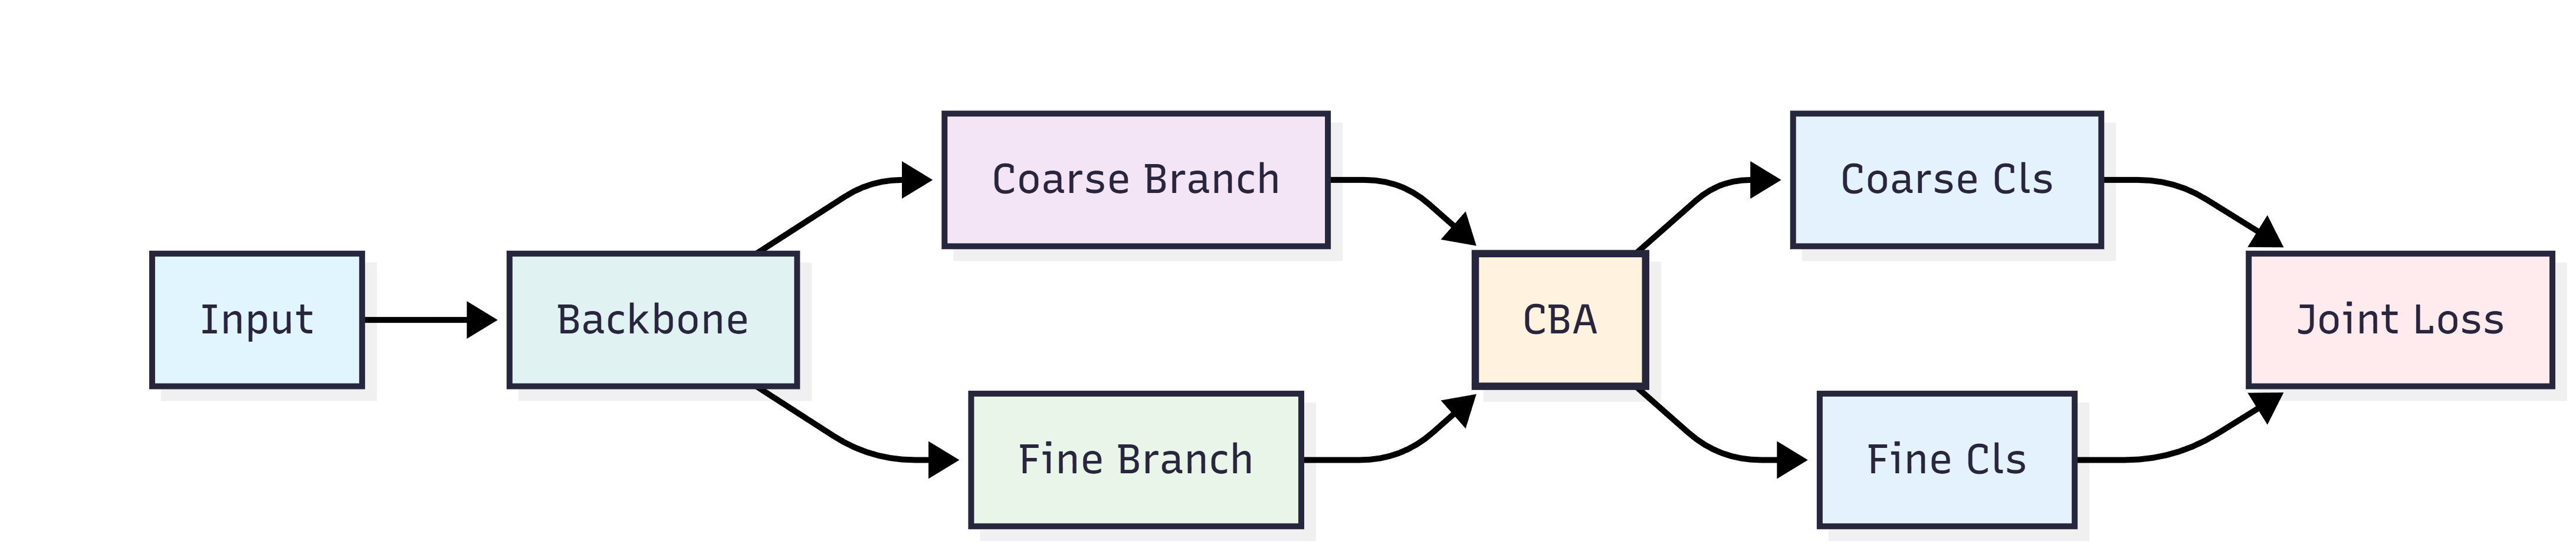
\includegraphics[width=\columnwidth]{imgs/model.png}
    \caption{Overall architecture of HFENet.}
    \label{fig:architecture}
\end{figure}


\subsection{Cross-Branch Attention Mechanism}
\label{sec:cba}

\subsubsection{Design Motivation}

Conventional attention modules such as SE and CBAM mainly recalibrate features within the same branch. Although effective for enhancing local saliency, they do not explicitly model the directional dependency that coarse-grained semantics should constrain fine-grained discrimination in hierarchical recognition tasks. Simple feature concatenation or linear fusion is also insufficient, because it lacks adaptive conditioning and may introduce redundant information sharing across branches.

To address this issue, we design a cross-branch attention mechanism that uses coarse-level semantics as conditional guidance for fine-grained feature modulation. From an information conditioning perspective, this mechanism can be interpreted as increasing the discriminative utility of fine-grained representations under the guidance of coarse semantics:
\begin{equation}
I(\mathbf{F}_f'; y_f \mid \mathbf{F}_c),
\end{equation}
where $\mathbf{F}_f'$ denotes the modulated fine-grained features.

\subsubsection{Mechanism Implementation}
To enable conditional semantic guidance, we design a cross-branch attention module that uses coarse features to modulate fine features. The coarse feature $\mathbf{F}_c$ is compressed into a channel attention vector $\mathbf{a}_c \in \mathbb{R}^C$ and a spatial attention map $\mathbf{A}_s \in \mathbb{R}^{H \times W \times 1}$. These are combined via outer product to form a modulation mask:
\begin{equation}
\mathbf{M} = 1 + \alpha \cdot (\mathbf{a}_c \otimes \mathbf{A}_s),
\label{eq:attention_mask}
\end{equation}
where $\alpha$ is a learnable scalar. The fine-grained feature is then modulated as:
\begin{equation}
\mathbf{F}_f' = \mathbf{F}_f \odot \mathbf{M}.
\label{eq:feature_modulation}
\end{equation}
This process implements spatially- and channel-wise adaptive guidance from the coarse branch to the fine branch.

\subsubsection{Comparison with Existing Attention Mechanisms}
To highlight the distinctiveness of our cross-branch attention, Table~\ref{tab:attention_comparison} compares it with several representative attention mechanisms.
\begin{table*}[htbp]
    \centering
    \caption{Comparison of CBA with representative attention mechanisms.}
    \label{tab:attention_comparison}
    \setlength{\tabcolsep}{4pt}
    \renewcommand{\arraystretch}{1.1}
    \small
    \begin{tabular}{@{}lccccc@{}}
    \toprule
    \textbf{Method} & \textbf{Input} & \textbf{Target} & \textbf{Hier.} & \textbf{Dyn.} & \textbf{Cost} \\
    \midrule
    SE-Net      & Single     & Same  & No   & Static  & $O(c^2/r)$ \\
    CBAM        & Single     & Same  & No   & Static  & $O(c^2/r + hwc)$ \\
    Non-local   & Single     & Same  & No   & Dynamic & $O((hw)^2c)$ \\
    Cross-attn. & Two-branch & Other & Weak & Dynamic & $O(hwc^2)$ \\
    \midrule
    \textbf{CBA (Ours)} & \textbf{Cross-level} & \textbf{Fine} & \textbf{Strong} & \textbf{Dynamic} & $\mathbf{O(c^2/r + hwc)}$ \\
    \bottomrule
    \end{tabular}
\end{table*}
As summarized in Table~\ref{tab:attention_comparison}, existing attention mechanisms mainly operate within a single branch or do not explicitly encode coarse-to-fine hierarchical conditioning. In contrast, the proposed CBA is designed for cross-branch modulation, where coarse-level semantics provide adaptive channel-spatial guidance to fine-grained representations.

\subsection{Orthogonality Regularization}
\label{sec:orth}
A dual-branch architecture does not automatically guarantee complementary representation learning. 
When both branches are optimized on the same input and related supervision signals, they may converge to overlapping feature subspaces, which weakens the benefit of hierarchical decomposition. 
Therefore, redundancy suppression is not merely an optional regularization term, but a necessary constraint for preserving functional differentiation between the coarse and fine branches.

To reduce cross-branch redundancy, we impose orthogonality between the coarse and fine features. For a batch of $N$ samples, let $\mathbf{F}_c \in \mathbb{R}^{N \times d_c}$ and $\mathbf{F}_f \in \mathbb{R}^{N \times d_f}$. The orthogonality loss is defined as:
\begin{equation}
\mathcal{L}_{\text{orth}} = \left\| \frac{1}{N}\mathbf{F}_c^\top \mathbf{F}_f - \text{diag}\left(\frac{1}{N}\mathbf{F}_c^\top \mathbf{F}_f\right) \right\|_F^2.
\label{eq:orth_loss}
\end{equation}
This penalty suppresses cross-branch correlation beyond the diagonal terms, thereby discouraging duplicated responses across the two branches. As a result, the coarse and fine branches are encouraged to encode complementary rather than redundant information, which is particularly important in dual-branch architectures with shared low-level features.

\subsection{Hierarchical Joint Optimization}
The overall loss function combines fine-grained classification loss $\mathcal{L}_f$, coarse-grained classification loss $\mathcal{L}_c$, hierarchical KL consistency loss $\mathcal{L}_{\mathrm{KL}}$, and orthogonality regularization:
\begin{equation}
\mathcal{L}_{\text{total}} = \mathcal{L}_f + \lambda_c \mathcal{L}_c + \lambda_{\mathrm{KL}} \mathcal{L}_{\mathrm{KL}} + \lambda_{\mathrm{orth}} \mathcal{L}_{\mathrm{orth}},
\label{eq:total_loss}
\end{equation}
where $\lambda_c$, $\lambda_{\mathrm{KL}}$, and $\lambda_{\mathrm{orth}}$ are balancing hyperparameters.

The complete training procedure is detailed in Algorithm~\ref{alg:training}.

\begin{algorithm}[t]
    \caption{Training procedure of HFENet}
    \label{alg:training}
    \begin{algorithmic}[1]
    \Require Training set $\mathcal{D}=\{(\mathbf{x}_i, y_{c,i}, y_{f,i})\}_{i=1}^N$, hyperparameters $\lambda_c$, $\lambda_{\mathrm{KL}}$, $\lambda_{\mathrm{orth}}$
    \Ensure Trained model parameters $\theta$
    \State Initialize network parameters $\theta$, optimizer AdamW ($\beta_1=0.9$, $\beta_2=0.999$, weight decay=5e-4)
    \State Set initial learning rate $\eta_0 = 0.001$, cosine annealing scheduler
    \For{$epoch = 1$ \textbf{to} $T$}
        \State Update learning rate: $\eta = \eta_0 \times \frac{1}{2}\left(1 + \cos\left(\frac{epoch}{T}\pi\right)\right)$
        \For{each mini-batch $\mathcal{B} = \{(\mathbf{X}_i, y_{c,i}, y_{f,i})\}_{i=1}^{B}$}
            \State $\mathbf{F}_s \gets \text{Backbone}(\mathbf{X})$
            \State $\mathbf{F}_c, \mathbf{F}_f \gets \text{Branch}_c(\mathbf{F}_s), \text{Branch}_f(\mathbf{F}_s)$
            \State $\mathbf{M} \gets \text{CBA}(\mathbf{F}_c, \mathbf{F}_f)$
            \State $\mathbf{F}_f' \gets \mathbf{F}_f \odot \mathbf{M}$
            \State $\hat{\mathbf{y}}_c, \hat{\mathbf{y}}_f \gets \text{Classifier}_c(\mathbf{F}_c), \text{Classifier}_f(\mathbf{F}_f')$
            \State $\mathcal{L}_{\text{total}} \gets \mathcal{L}_f(\hat{\mathbf{y}}_f, \mathbf{y}_f) + \lambda_c \mathcal{L}_c(\hat{\mathbf{y}}_c, \mathbf{y}_c) + \lambda_{\mathrm{KL}} \mathcal{L}_{\mathrm{KL}} + \lambda_{\mathrm{orth}} \mathcal{L}_{\mathrm{orth}}$
            \State Update $\theta$ using AdamW
        \EndFor
    \EndFor
    \State \Return $\theta$
    \end{algorithmic}
\end{algorithm}

\section{Experiments}
\label{sec:experiments}

\subsection{Datasets and Evaluation Metrics}
We evaluate on CIFAR-100 and Stanford Cars. CIFAR-100 contains 100 fine classes grouped into 20 coarse super-classes. Stanford Cars contains 196 fine classes (car models) with coarse labels based on brand (49 brands). We use 30\%, 50\%, 80\%, and 100\% training ratios to evaluate data efficiency. Top-1 accuracy (\%) is reported as mean $\pm$ std over three runs.

\subsection{Implementation Details}
All models are implemented in PyTorch and trained from scratch. Backbone: WideResNet-16-8 for HFENet and baselines. Optimizer: AdamW (lr=0.001, weight decay=5e-4) with cosine annealing for 300 epochs. Batch size: 64. Data augmentation: random cropping, horizontal flipping, AutoAugment, and random erasing (p=0.5). Loss weights: $\lambda_c=0.5$, $\lambda_{\mathrm{KL}}=0.2$, $\lambda_{\mathrm{orth}}=0.0005$ (determined via grid search).

\subsection{Comparison with State-of-the-Art}
Under a unified from-scratch training protocol, HFENet achieves stronger performance than representative Transformer backbones in limited-data settings. 
This result suggests that the proposed hierarchical inductive bias is more data-efficient under small- to medium-scale supervision.
It should be noted that all comparison models are trained under the same from-scratch protocol for fairness. Therefore, the results should be interpreted primarily as a comparison of data efficiency under a unified training regime, rather than as a universal ranking across different model families.

\begin{table*}[htbp]
    \centering
    \caption{Classification accuracy (\%) on CIFAR-100 under different training ratios.}
    \label{tab:cifar100_data_ratio}
    \begin{tabular}{@{}lcccc@{}}
    \toprule
    \textbf{Method} & \textbf{30\% data} & \textbf{50\% data} & \textbf{80\% data} & \textbf{100\% data} \\
    \midrule
    WRN-16-8 (Baseline) & 58.4 ± 0.3 & 68.7 ± 0.4 & 76.3 ± 0.2 & 80.2 ± 0.2 \\
    Dual-branch WRN (no interaction) & 61.6 ± 0.4 & 70.7 ± 0.3 & 78.2 ± 0.3 & 80.6 ± 0.2 \\
    ResNet50 & 55.2 ± 0.5 & 64.8 ± 0.4 & 72.5 ± 0.3 & 76.8 ± 0.3 \\
    DenseNet121 & 57.6 ± 0.4 & 66.9 ± 0.3 & 74.1 ± 0.3 & 78.3 ± 0.2 \\
    EfficientNet-B0 & 56.8 ± 0.5 & 66.2 ± 0.4 & 73.7 ± 0.3 & 77.9 ± 0.3 \\
    ViT-B & 39.5 ± 0.7 & 49.4 ± 0.6 & 64.6 ± 0.4 & 69.7 ± 0.4 \\
    Swin-T & 52.7 ± 0.6 & 59.7 ± 0.5 & 66.2 ± 0.4 & 69.1 ± 0.3 \\
    PVTv2 & 48.3 ± 0.6 & 56.9 ± 0.5 & 63.8 ± 0.4 & 67.5 ± 0.4 \\
    ConvNeXt-V2 & 53.8 ± 0.5 & 62.4 ± 0.4 & 69.1 ± 0.3 & 72.6 ± 0.3 \\
    \hline
    \textbf{HFENet (Ours)} & \textbf{70.8 ± 0.3} & \textbf{77.2 ± 0.2} & \textbf{80.5 ± 0.2} & \textbf{82.7 ± 0.2} \\
    \bottomrule
    \end{tabular}
\end{table*}

Results in Table~\ref{tab:cifar100_data_ratio} show that HFENet consistently outperforms all baselines, especially under limited data. At 30\% data, it improves over WRN-16-8 by 12.4\%, and at 100\% data by 2.5\%. Notably, at 50\% data, HFENet already surpasses the full-data performance of WRN-16-8.

\subsubsection{Convergence Analysis}
Convergence curves in Fig.~\ref{fig:convergence_curves} further illustrate the optimization behavior. HFENet achieves faster initial convergence and better final accuracy, demonstrating the benefit of hierarchical guidance and redundancy suppression.
\begin{figure*}[htbp]
    \centering
    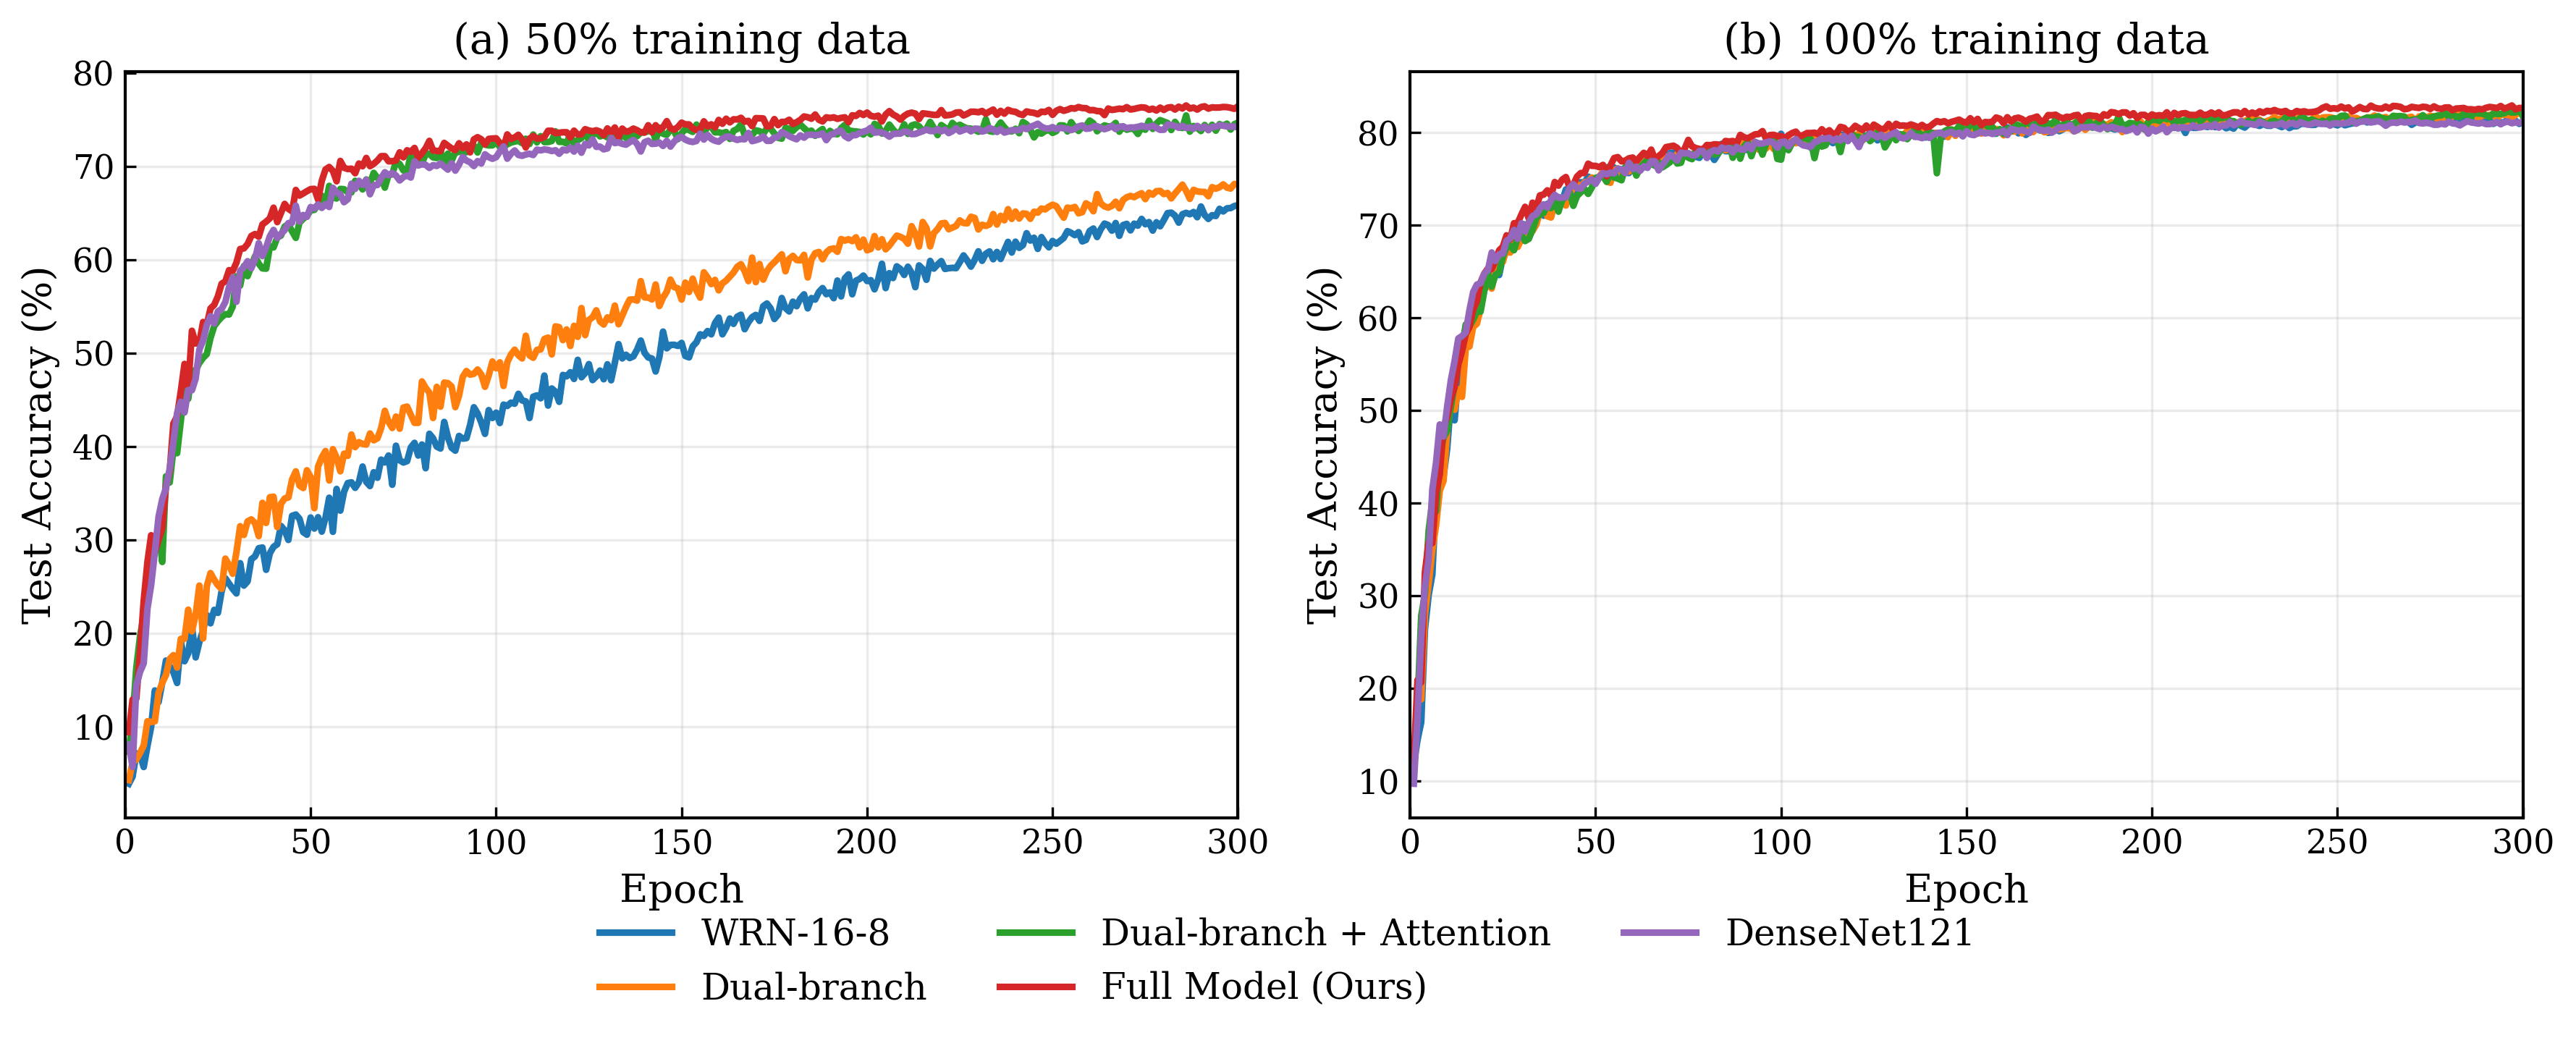
\includegraphics[width=\textwidth]{imgs/convergence_curves_final_paper.png}
    \caption{Test accuracy convergence curves on CIFAR-100 with 50\% and 100\% training data.}
    \label{fig:convergence_curves}
\end{figure*}

\subsection{Results on Stanford Cars}
To provide preliminary evidence of generalizability, we further evaluate HFENet on Stanford Cars, an additional fine-grained benchmark with 196 model classes and 49 brand-level coarse categories. Results are shown in Table~\ref{tab:cars_results}.
\begin{table*}[htbp]
    \centering
    \caption{Classification accuracy (\%) on Stanford Cars.}
    \label{tab:cars_results}
    \begin{tabular}{@{}lcc@{}}
    \toprule
    \textbf{Method} & \textbf{50\% data} & \textbf{100\% data} \\
    \midrule
    WRN-16-8 (Baseline) & 50.52 ± 0.6 & 81.17 ± 0.3 \\
    Dual-branch WRN (no interaction) & 62.48 ± 0.5 & 82.24 ± 0.3 \\
    Dual-branch + CBA & 63.25 ± 0.4 & 83.04 ± 0.2 \\
    \textbf{HFENet (Ours)} & \textbf{65.73 ± 0.4} & \textbf{83.95 ± 0.2} \\
    \hline
    ResNet50 & 42.07 ± 0.7 & 80.06 ± 0.4 \\
    DenseNet121 & 49.12 ± 0.6 & 82.31 ± 0.3 \\
    \bottomrule
    \end{tabular}
\end{table*}
HFENet achieves the highest accuracy among the compared methods in both data settings, providing preliminary evidence that the proposed hierarchical alignment strategy can generalize to an additional fine-grained benchmark.

\subsection{Ablation Studies}
We conduct ablations on CIFAR-100 to isolate the contribution of each component. Results are presented in Table~\ref{tab:ablation_all}.

\begin{table*}[htbp]
    \centering
    \caption{Ablation results on CIFAR-100 under different training ratios (\% accuracy).}
    \label{tab:ablation_all}
    \setlength{\tabcolsep}{4pt}
    \renewcommand{\arraystretch}{1.1}
    \small
    \begin{tabular}{@{}lccccc@{}}
    \toprule
    \textbf{Ratio} & \textbf{WRN-16-8} & \textbf{Dual} & \textbf{Dual+CBA} & \textbf{Dual+Orth.} & \textbf{Full} \\
    \midrule
    30\%  & 58.4 $\pm$ 0.3 & 61.6 $\pm$ 0.4 & 69.9 $\pm$ 0.3 & 62.3 $\pm$ 0.2 & \textbf{70.8 $\pm$ 0.3} \\
    50\%  & 68.7 $\pm$ 0.4 & 70.7 $\pm$ 0.3 & 75.3 $\pm$ 0.3 & 71.2 $\pm$ 0.3 & \textbf{77.2 $\pm$ 0.2} \\
    80\%  & 76.3 $\pm$ 0.2 & 78.2 $\pm$ 0.3 & 79.2 $\pm$ 0.2 & 78.8 $\pm$ 0.2 & \textbf{80.5 $\pm$ 0.2} \\
    100\% & 80.2 $\pm$ 0.2 & 80.6 $\pm$ 0.2 & 82.1 $\pm$ 0.2 & 81.2 $\pm$ 0.2 & \textbf{82.7 $\pm$ 0.2} \\
    \bottomrule
    \end{tabular}
\end{table*}

Dual-branch decomposition alone yields limited improvements over the baseline, indicating that merely separating coarse- and fine-level pathways is insufficient. 
Introducing CBA brings substantial gains, which confirms the importance of explicit coarse-to-fine semantic guidance. 
Adding orthogonality regularization further improves performance by suppressing redundant cross-branch representations. 
The full model achieves the best results across all training ratios, suggesting that hierarchical alignment and redundancy suppression are complementary rather than interchangeable.

\subsection{Feature Correlation Analysis}
Feature correlation analysis. Orthogonality regularization reduces cross-branch feature redundancy.

\begin{figure}[H]
    \centering
    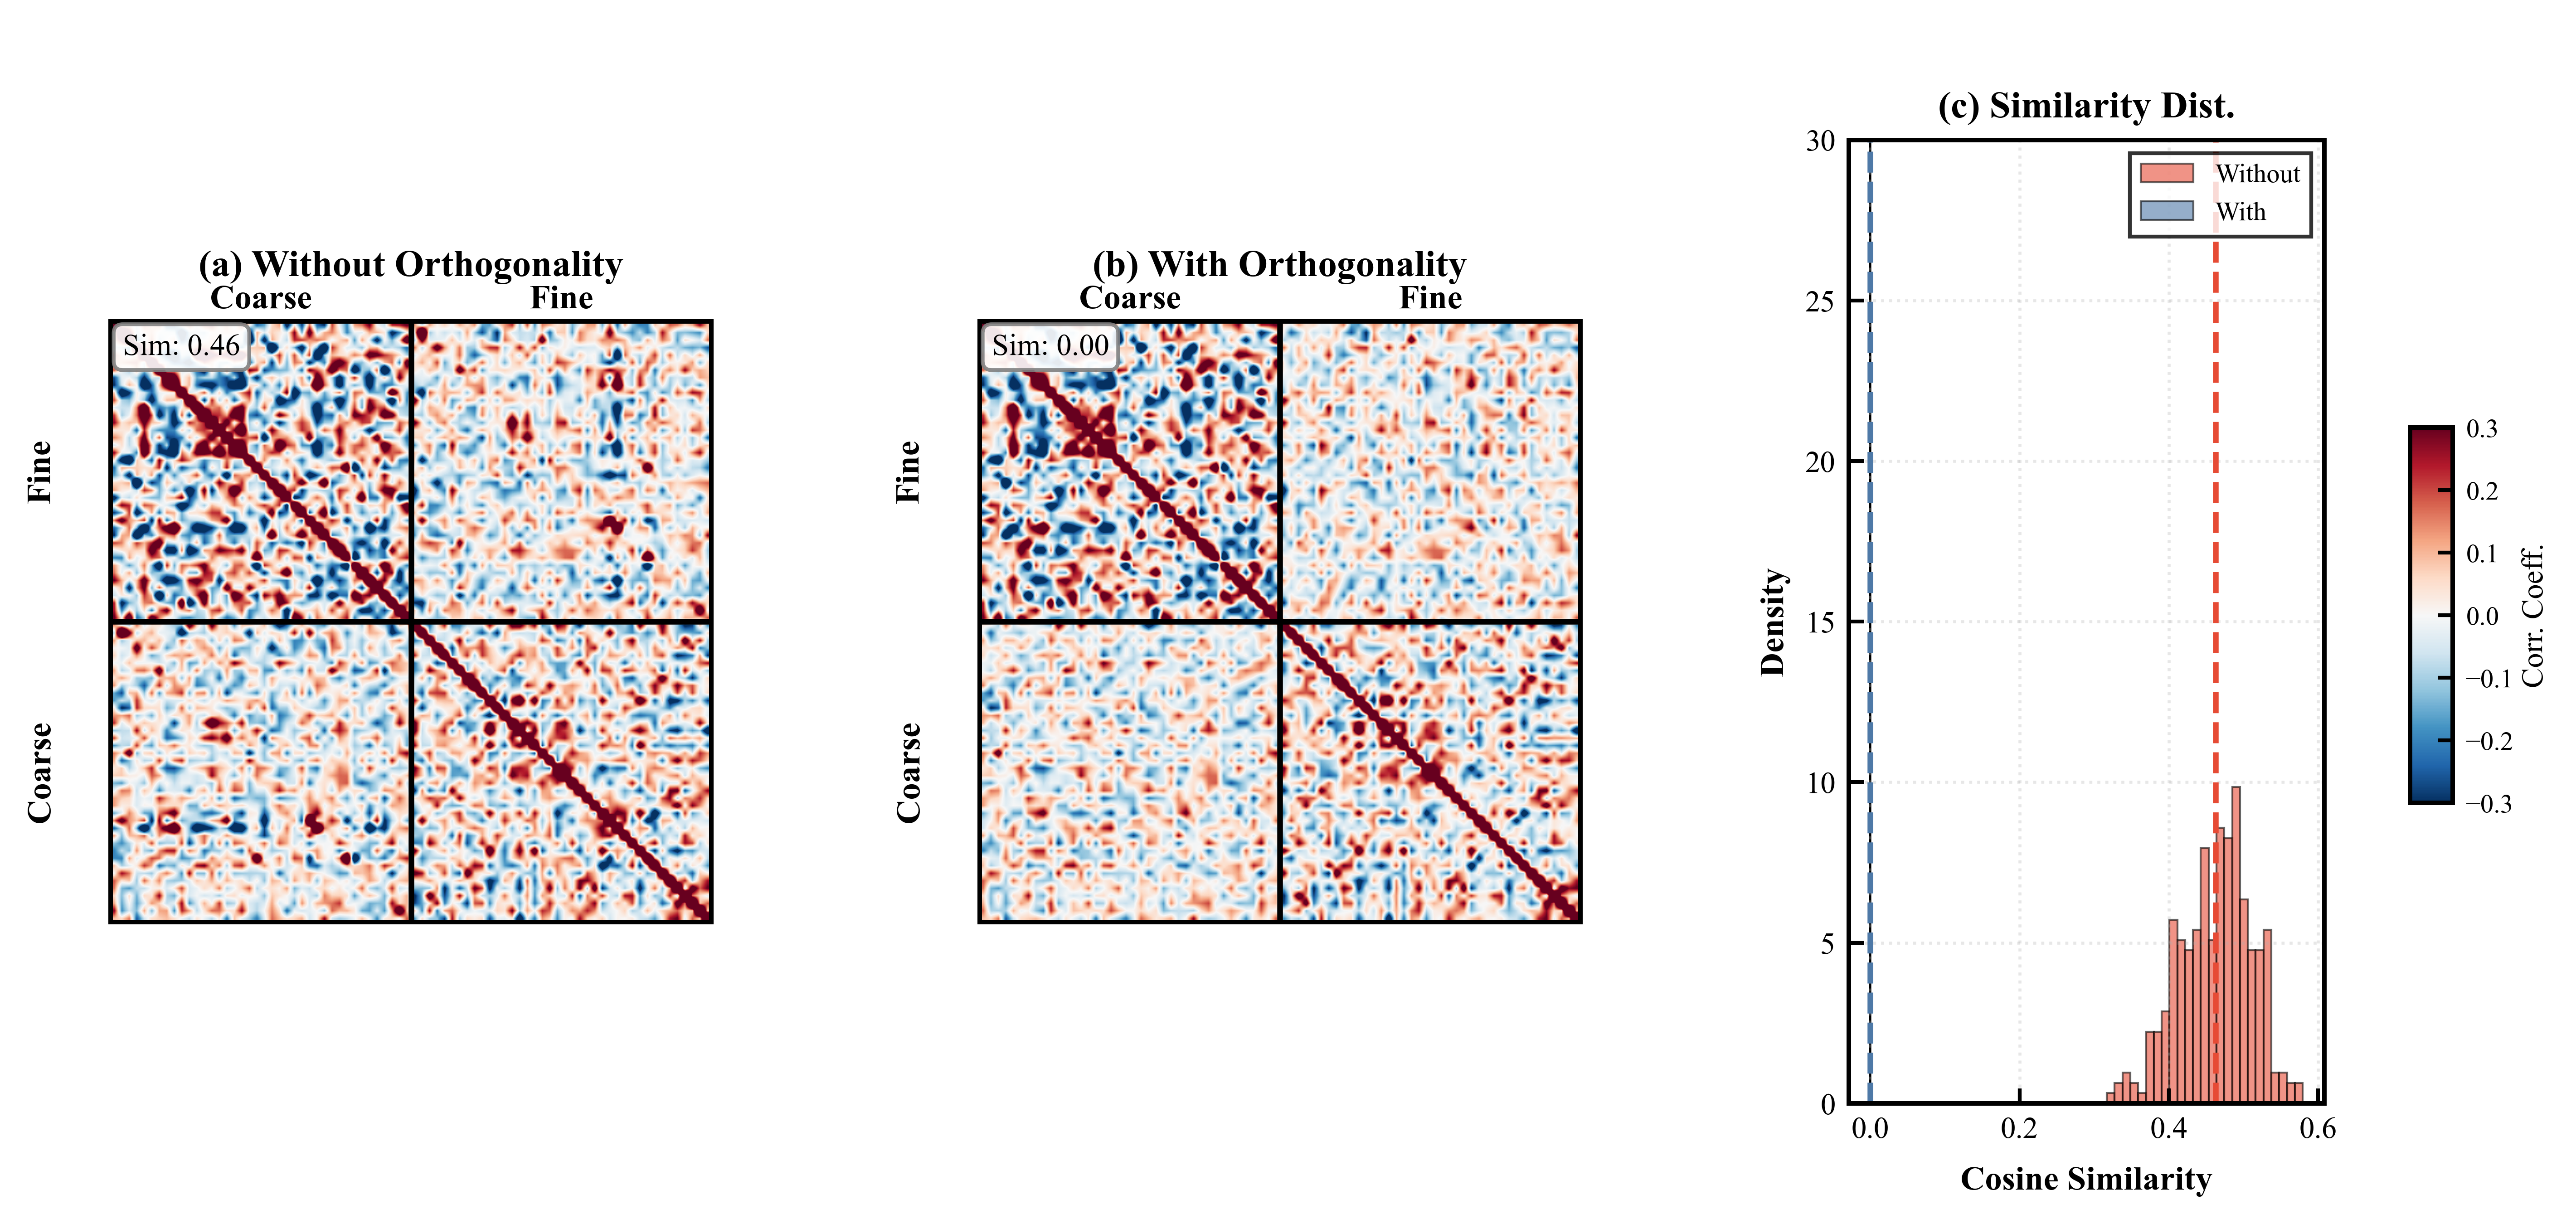
\includegraphics[width=0.9\columnwidth]{imgs/fig2_combined.png}
    \caption{Feature correlation analysis of dual-branch representations with and without orthogonality regularization.}
\end{figure}
The reduced correlation indicates that the two branches learn less redundant and more complementary representations, which is consistent with the role of orthogonality regularization in suppressing branch-wise overlap.

\FloatBarrier

\subsection{Visualization Analysis}
We visualize Grad-CAM heatmaps on CIFAR-100 (Fig.~\ref{fig:grad_cam_vis}) and Stanford Cars (Fig.~\ref{fig:cars_gradcam}) to examine the qualitative effect of hierarchical feature alignment. Compared with WRN-16-8, HFENet tends to produce more target-focused responses with less distraction from irrelevant regions.

\begin{figure*}[!b]
    \centering
    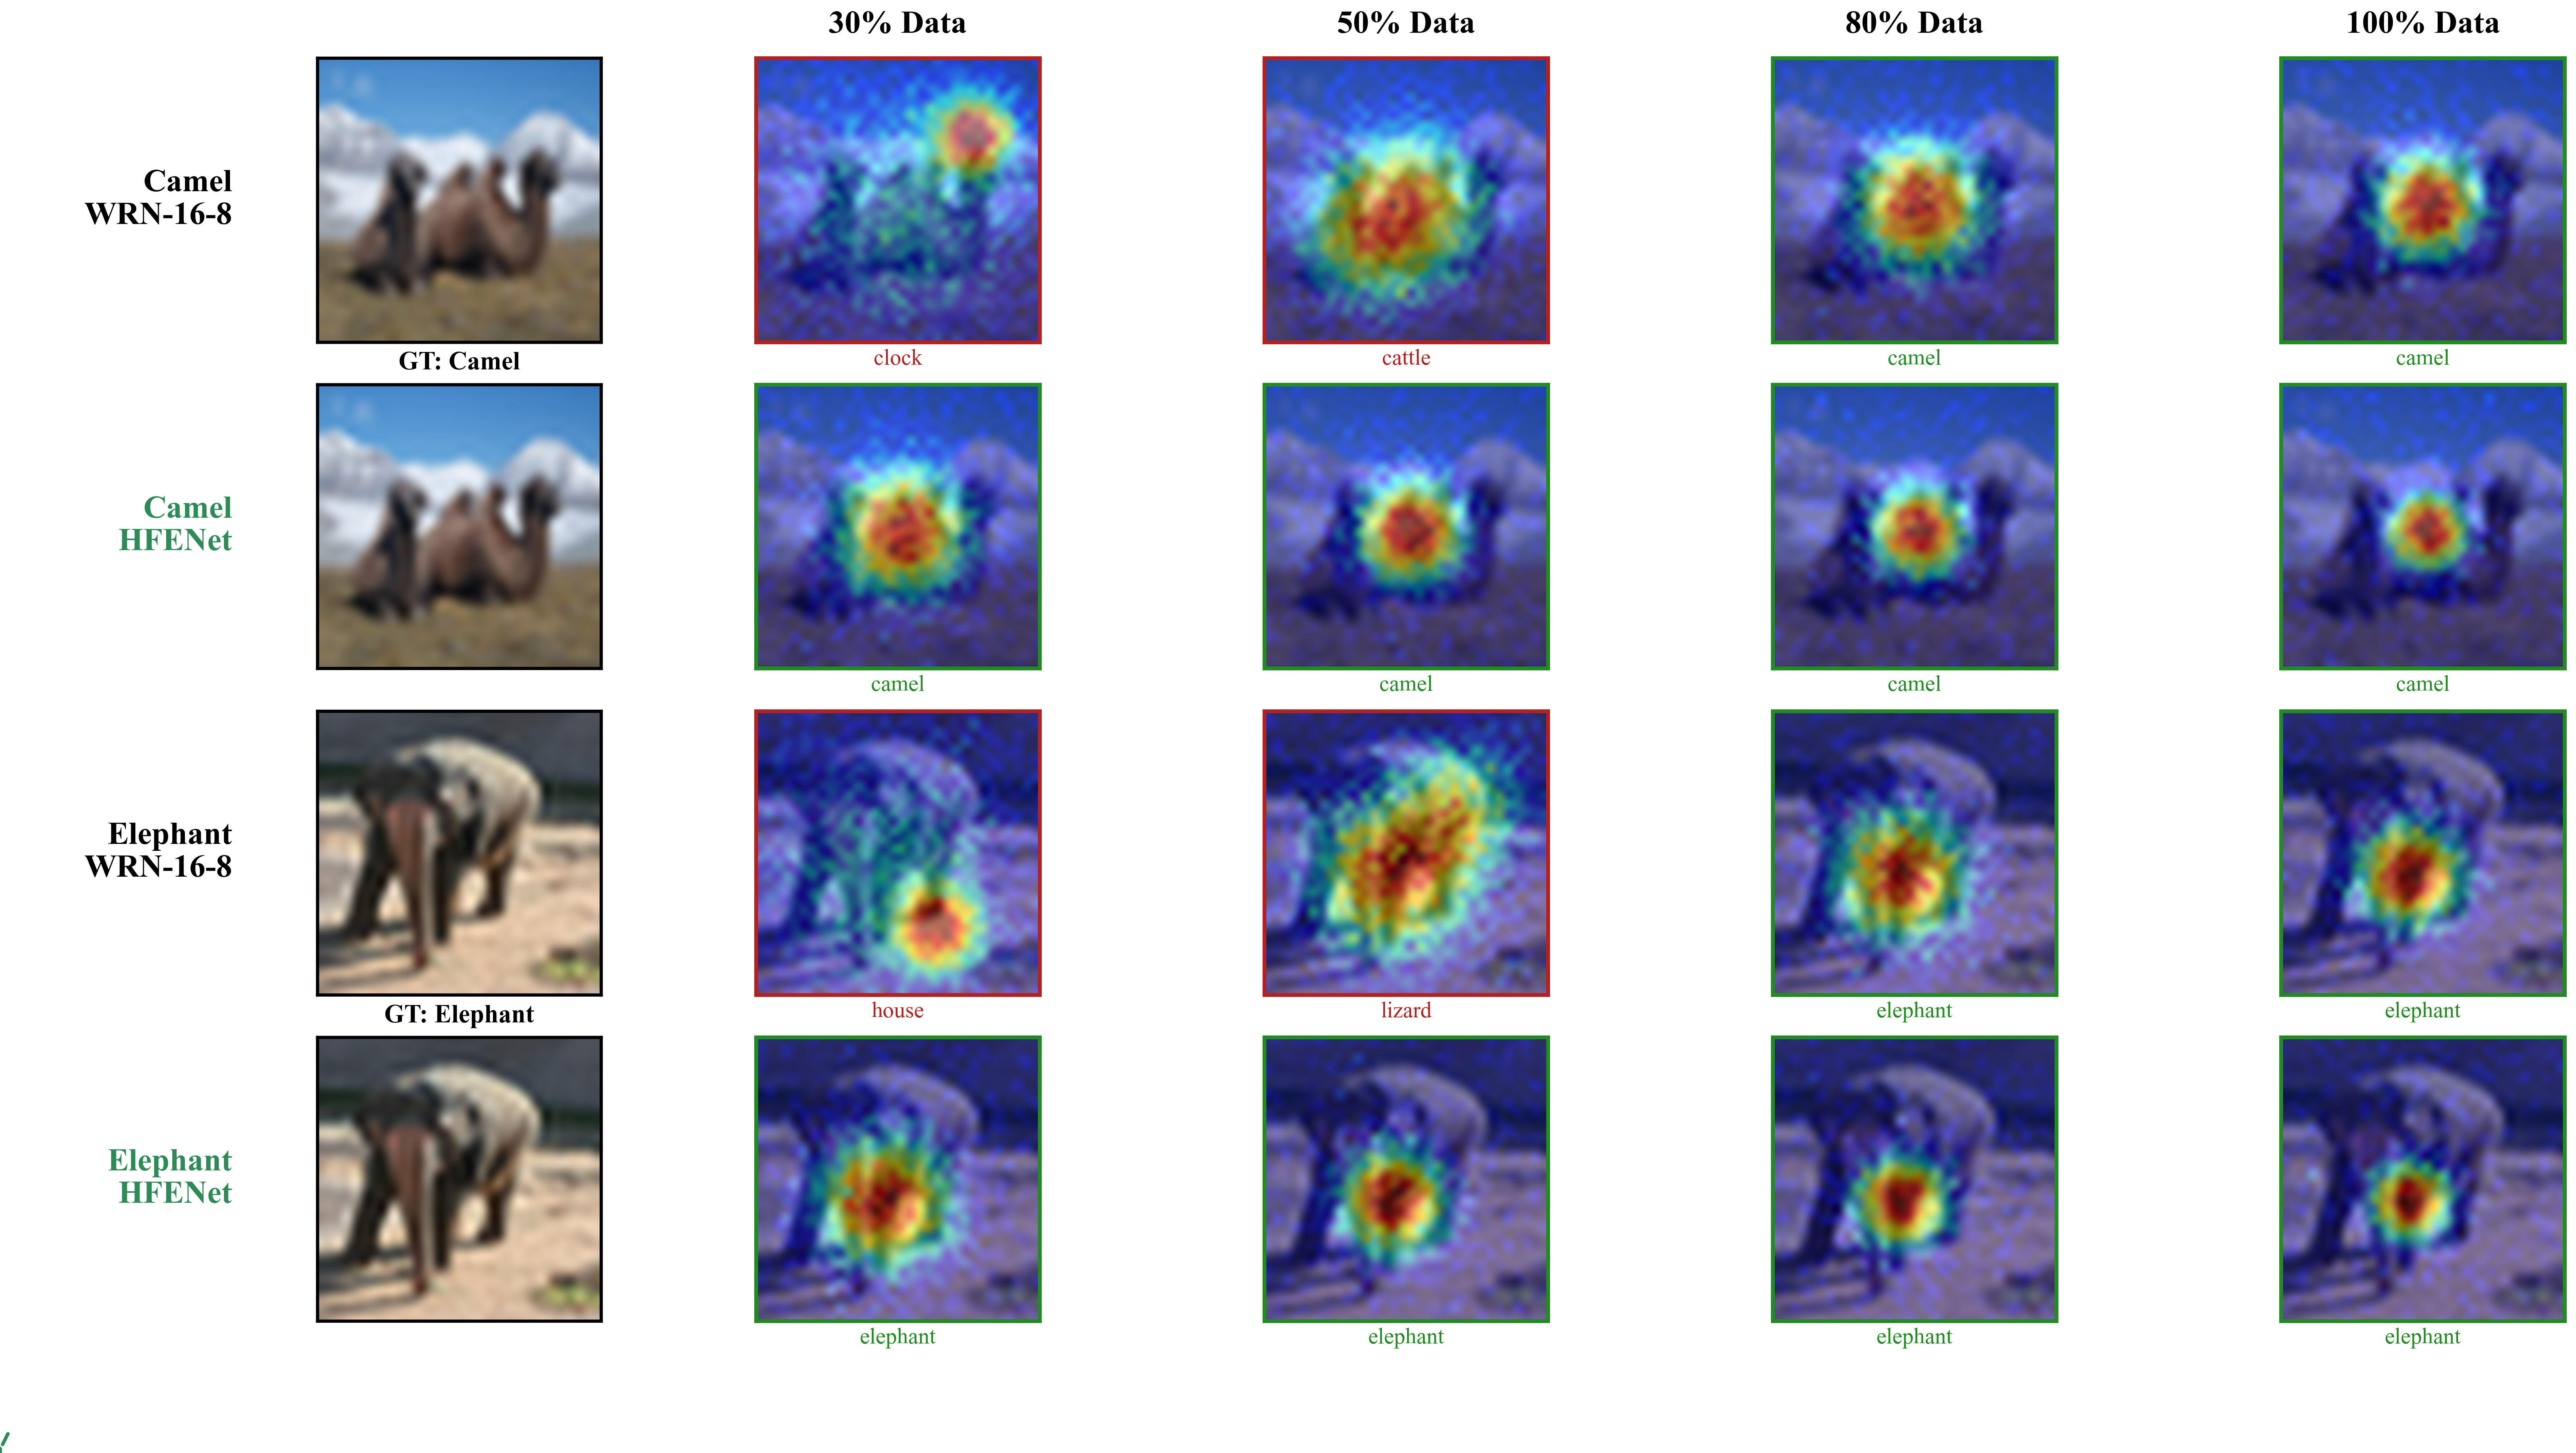
\includegraphics[width=\textwidth]{imgs/fig3_sci_q4_comparison_two_classes.png}
    \caption{Grad-CAM comparison between WRN-16-8 and HFENet on CIFAR-100 under different training ratios.}    \label{fig:grad_cam_vis}
\end{figure*}

This trend is more evident under reduced training ratios, where coarse-to-fine semantic guidance appears to improve the stability of discriminative localization.


\begin{figure}[!b]
    \centering
    \includegraphics[width=\columnwidth]{imgs/fig3_stanford_cars_two_classes.png}
    \caption{Grad-CAM comparison between WRN-16-8 and HFENet on Stanford Cars.}
        \label{fig:cars_gradcam}
\end{figure}
\FloatBarrier

\subsection{Error Analysis}
We analyze misclassifications of HFENet on CIFAR-100. We further inspect representative failure cases of HFENet on CIFAR-100. Most errors are associated with one of three challenging conditions: severe occlusion of key parts, extremely subtle inter-class differences, and low-resolution images with insufficient local detail. These cases suggest that, although hierarchical guidance improves discriminative focus, the model remains sensitive to missing part cues and limited visual resolution.

\section{Discussion}
\label{sec:discussion}

\subsection{Advantages of the Proposed Method}
HFENet improves data efficiency by jointly addressing two issues in hierarchical fine-grained learning: insufficient semantic coordination across levels and feature redundancy across branches. The proposed cross-branch attention allows coarse-level semantics to condition fine-grained feature modulation, which helps stabilize discriminative learning when training data are limited. Meanwhile, orthogonality regularization reduces redundant responses between the two branches and encourages a more complementary division of representation roles. Taken together, these two components provide a structured way to couple semantic guidance with redundancy suppression in dual-branch fine-grained classification.

\subsection{Practical Application Scenarios}
HFENet is particularly suitable for scenarios with natural or definable category hierarchies and limited training samples. Potential applications include:
\begin{itemize}
    \item Industrial defect inspection, where product categories are naturally hierarchical (e.g., type of defect, severity level) and labeled data is often scarce.
    \item Species recognition in biology, where coarse taxonomic ranks (genus, family) can guide fine-grained species identification.
    \item Fine-grained product recognition in e-commerce, where brand-level semantics help differentiate similar models.
\end{itemize}
It is worth noting that this work does not systematically evaluate efficiency in resource-constrained deployment (e.g., edge devices), and its practical applicability in such settings remains for future investigation.

\subsection{Limitations and Future Work}
Current limitations include:
\begin{itemize}
    \item Reliance on predefined hierarchical labels; the method may not directly apply when such labels are absent.
    \item Introduction of additional hyperparameters ($\lambda_c$, $\lambda_{\mathrm{KL}}$, $\lambda_{\mathrm{orth}}$), which require tuning on a validation set.
    \item Evaluation is limited to CIFAR-100 and Stanford Cars; broader fine-grained datasets (e.g., iNaturalist, NABirds) should be tested.
\end{itemize}
Future work will focus on: (1) extending the framework to more diverse fine-grained benchmarks; (2) exploring adaptive or self-supervised hierarchy discovery; (3) designing more efficient implementations of attention and orthogonality constraints; (4) transferring the hierarchical alignment idea to other vision tasks such as object detection and segmentation; and (5) investigating semi-supervised or weakly-supervised settings where hierarchy labels are only partially available.

\section{Conclusion}
\label{sec:conclusion}
This paper proposed HFENet, a dual-branch framework for fine-grained image classification built around the central idea of hierarchical feature alignment for coarse-to-fine representation learning. 
Within this framework, cross-branch attention enables directional semantic guidance from the coarse branch to the fine branch, while orthogonality regularization suppresses redundant cross-branch representations and promotes complementarity. 
Hierarchical KL consistency further improves semantic coherence during training. 
Experimental results on CIFAR-100 and Stanford Cars show that HFENet consistently improves recognition performance, especially under limited-data settings. 
These findings suggest that explicitly combining hierarchical alignment and redundancy suppression is a promising direction for data-efficient fine-grained recognition.

\section*{Acknowledgements}
We thank our laboratory colleagues for valuable discussions and the anonymous reviewers for their constructive comments. This work was supported by the XXX Foundation (Grant No. XXXX).

\begin{thebibliography}{50}

\bibitem{he2016deep} He, K., Zhang, X., Ren, S., \& Sun, J. (2016). Deep residual learning for image recognition. In \textit{Proceedings of the IEEE Conference on Computer Vision and Pattern Recognition} (pp. 770-778).

\bibitem{huang2017densely} Huang, G., Liu, Z., Van Der Maaten, L., \& Weinberger, K. Q. (2017). Densely connected convolutional networks. In \textit{Proceedings of the IEEE Conference on Computer Vision and Pattern Recognition} (pp. 4700-4708).

\bibitem{du2020fine} Du, R., Chang, D., Bhunia, A. K., Xie, J., Ma, Z., Song, Y. Z., \& Guo, J. (2020). Fine-grained visual classification via progressive multi-granularity training. In \textit{European Conference on Computer Vision} (pp. 137-153). Springer, Cham.

\bibitem{yan2015hdcnn} Yan, Z., Zhang, H., Piramuthu, R., Jagadeesh, V., DeCoste, D., Di, W., \& Yu, Y. (2015). HD-CNN: hierarchical deep convolutional neural network for large scale visual recognition. In \textit{Proceedings of the IEEE International Conference on Computer Vision} (pp. 2740-2748).

\bibitem{hu2018squeeze} Hu, J., Shen, L., \& Sun, G. (2018). Squeeze-and-excitation networks. In \textit{Proceedings of the IEEE Conference on Computer Vision and Pattern Recognition} (pp. 7138-7141).

\bibitem{woo2018cbam} Woo, S., Park, J., Lee, J. Y., \& Kweon, I. S. (2018). CBAM: Convolutional block attention module. In \textit{Proceedings of the European Conference on Computer Vision} (pp. 3-19).

\bibitem{zheng2017learning} Zheng, H., Fu, J., Mei, T., \& Luo, J. (2017). Learning multi-attention convolutional neural network for fine-grained image recognition. In \textit{Proceedings of the IEEE International Conference on Computer Vision} (pp. 5209-5217).

\bibitem{fu2017look} Fu, J., Zheng, H., \& Mei, T. (2017). Look closer to see better: Recurrent attention convolutional neural network for fine-grained image recognition. In \textit{Proceedings of the IEEE Conference on Computer Vision and Pattern Recognition} (pp. 4438-4446).

\bibitem{xnet2019} Chen, Y., Li, J., Xiao, H., Jin, X., Yan, S., \& Feng, J. (2019). Dual path networks for multi-person human pose estimation. \textit{arXiv preprint arXiv:1902.07424}.

\bibitem{he2021transfg} He, J., Chen, J. N., Liu, S., Kortylewski, A., Yang, C., Bai, Y., \& Wang, C. (2021). Transfg: A transformer architecture for fine-grained recognition. In \textit{Proceedings of the AAAI Conference on Artificial Intelligence} (Vol. 36, No. 1, pp. 852-860).

\bibitem{yang2018nested} Yang, Z., Luo, T., Wang, D., Hu, Z., Gao, J., \& Wang, L. (2018). Learning to navigate for fine-grained classification. In \textit{Proceedings of the European Conference on Computer Vision} (pp. 420-435).

\bibitem{part_rcnn} Zhang, N., Donahue, J., Girshick, R., \& Darrell, T. (2014). Part-based R-CNNs for fine-grained category detection. In \textit{European Conference on Computer Vision} (pp. 834-849). Springer, Cham.

\bibitem{bilinear_cnn} Lin, T. Y., RoyChowdhury, A., \& Maji, S. (2015). Bilinear CNN models for fine-grained visual recognition. In \textit{Proceedings of the IEEE International Conference on Computer Vision} (pp. 1449-1457).

\bibitem{nonlocal} Wang, X., Girshick, R., Gupta, A., \& He, K. (2018). Non-local neural networks. In \textit{Proceedings of the IEEE Conference on Computer Vision and Pattern Recognition} (pp. 7794-7803).

\bibitem{dosovitskiy2020image} Dosovitskiy, A., Beyer, L., Kolesnikov, A., Weissenborn, D., Zhai, X., Unterthiner, T., ... \& Houlsby, N. (2020). An image is worth 16x16 words: Transformers for image recognition at scale. \textit{arXiv preprint arXiv:2010.11929}.

\bibitem{liu2021swin} Liu, Z., Lin, Y., Cao, Y., Hu, H., Wei, Y., Zhang, Z., ... \& Guo, B. (2021). Swin transformer: Hierarchical vision transformer using shifted windows. In \textit{Proceedings of the IEEE/CVF International Conference on Computer Vision} (pp. 10012-10022).

\bibitem{touvron2021training} Touvron, H., Cord, M., Douze, M., Massa, F., Sablayrolles, A., \& Jégou, H. (2021). Training data-efficient image transformers \& distillation through attention. In \textit{International Conference on Machine Learning} (pp. 10347-10357). PMLR.

\bibitem{liu2022convnext} Liu, Z., Mao, H., Wu, C. Y., Feichtenhofer, C., Darrell, T., \& Xie, S. (2022). A convnet for the 2020s. In \textit{Proceedings of the IEEE/CVF Conference on Computer Vision and Pattern Recognition} (pp. 11976-11986).

\bibitem{wang2022pvt} Wang, W., Xie, E., Li, X., Fan, D. P., Song, K., Liang, D., ... \& Shao, L. (2022). PVT v2: Improved baselines with pyramid vision transformer. \textit{Computational Visual Media}, 8(3), 415-424.

\bibitem{liu2022swinv2} Liu, Z., Hu, H., Lin, Y., Yao, Z., Xie, Z., Wei, Y., ... \& Guo, B. (2022). Swin transformer v2: Scaling up capacity and resolution. In \textit{Proceedings of the IEEE/CVF Conference on Computer Vision and Pattern Recognition} (pp. 12009-12019).

\bibitem{woo2023convnextv2} Woo, S., Debnath, S., Hu, R., Chen, X., Liu, Z., Kweon, I. S., \& Xie, S. (2023). ConvNeXt V2: Co-designing and scaling ConvNets with masked autoencoders. In \textit{Proceedings of the IEEE/CVF Conference on Computer Vision and Pattern Recognition} (pp. 16133--16142).

\end{thebibliography}

\end{document}